\subsection{Software Architecture}

\todo[inline]{FIX THE BELOW REFERENCES!!!!}

Since we use a microcontroller from Energy Micro, which in turn is a Cortex
microcontroller, the software is based on the CMSIS \ref{CMSIS} codebase from
ARM. The Giant Gecko MCU is supplied with a peripheral application programming
interface (API), called emlib \ref{emlib} which builds upon CMSIS and can be
used to initialize and control all attached peripherals. The code and
programming model is based on how it is done in emlib, and have mostly used the
emlib API for communicating and controlling the microcontoller.

\begin{figure}[H]
    \centering
    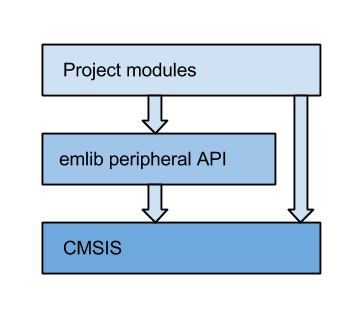
\includegraphics[height=150px]{figures/sw/software-stack.png}
    \caption{The software stack used on the microcontroller}
    \label{fig:software-stack}
\end{figure}


The application code is structured into directories representing each of the
modules, or peripherals, which we have written custom software for. Each module
\todo{WHY?}contains three directories, \textit{inc}, \textit{src} and \textit{demo}. Each
of these directories contains header files, source files and different demos or
test programs for the modules, respectively. Each module is typically
implemented as a combination of a driver and a controller for the specific
device that it is designed for.
